\section{Funzioni di controllo di Ljapunov}
Per i sistemi non lineari esiste un criterio che permette di determinarne
la controllabilità asintotica, chiamato \emph{metodo di Ljapunov}.
L'idea è di trovare una \emph{energia generalizzata} $V(\b x)$
che sia sempre decrescente nel tempo,
così che il sistema tenda a minimizzarla.
La difficoltà sta nel trovare una funzione di Lyapunov;
compito non facile, in generale, e per cui spesso è richiesta
una qualche forma di \emph{ispirazione Divina}~\cite{strogatz}.


Per usare i risultati della teoria di Ljapunov è necessario lavorare
con \emph{sistemi topologici}, una classe più ristretta di problemi di controllo.
Per quanto riguarda questo testo è sufficiente pensare a un sistema topologico
come un problema di controllo in cui la mappa di transizione è una funzione
continua.
% Anche qui citare sontag

\begin{definition}
    Un \textbf{sistema topologico} è un problema di controllo in
    cui lo spazio delle fasi $\Sigma$ è dotato di metrica e,
    dato $t \in \mathcal T$ e $\b x \in \Sigma$,
    vale la seguente proprietà:

    \emph{Se $\omega$ è un controllo ammesso per $\b x$ e la successione
    ${\b x_n}$ tende a $\b x$ allora deve esistere un intero
    $N$ tale che, preso $n \geq N$ allora $\omega$ è ammesso per $x_n$
    e il limite~\eqref{eq:def-sistema-topologico} converge uniformemente a $0$ per $s \in [0, t]$.}
    \begin{equation}
        \lim_{N \to +\infty} d[\phi^s(\b x_n, \omega), \phi^s(\b x, \omega)] = 0.
        \label{eq:def-sistema-topologico}
    \end{equation}
\end{definition}


Enuncio la definizione di \emph{funzione di controllo di Ljapunov}.
\begin{definition}
    \label{def:clf-local}
    Dato un problema di controllo in cui $\b x^*$ è un punto fisso e
    $\mathcal O$ è un intorno di $\b x^*$.
    Una funzione continua
    \begin{equation*}
        V : \Sigma \to \R,
    \end{equation*}
    è detta \textbf{funzione locale di controllo di Ljapunov} se
    e solo se valgono le seguenti proprietà:

    \begin{itemize}
        \item 1) $V$ è propria in $\b x^*$, ovvero l'insieme
        \begin{equation*}
            \left\{\b x \in \Sigma\ |\ V(\b x) \leq \epsilon \right\}
        \end{equation*}
        è un sottoinsieme compatto di $\mathcal O$ per ogni $\epsilon$ piccolo a piacere.
        \item 2) $V$ è definita positiva in $\mathcal O$, ovvero $V(\b x^*) = 0$ e
        $V(\b x) > 0$ per ogni $\b x \neq \b x^* \in \mathcal O$.
        \item 3) Per ogni $\b x \neq \b x^* \in \mathcal O$
        esiste un tempo $0 < t \in \mathcal T$ e un controllo $\omega \in \mathcal U^{[0,t[ \subseteq \mathcal T}$
        tali che, detta $\xi(s) = \phi^s(\b x, \omega)$, vale
        \begin{align*}
            V(\xi(s)) &\leq V(\b x) \text{ per ogni } s \in [0,t[ \subseteq \mathcal T, \\
            V(\xi(t)) &< V(\b x).
        \end{align*}
    \end{itemize}
\end{definition}

\begin{definition}
    Se nella \autoref{def:clf-local} l'intorno $\mathcal O$ coincide
    con tutto lo spazio delle fasi $\Sigma$ allora $V$ è una
    \textbf{funzione di controllo di Ljapunov}.
    \label{def:clf}
\end{definition}

Le Definizioni~\ref{def:clf-local} e~\ref{def:clf} valgono anche per sistemi
senza controlli; in questo caso $V$ è chiamata solamente \emph{funzione (locale) di Ljapunov}.
Il termine (\emph{locale}) tra parentesi indica che l'affermazione è da intendersi valida
sia che il termine \emph{locale} sia presente o meno.

\begin{definition}
    Sia $V$ una funzione (locale) di controllo di Ljapunov.
    Dati $\b x, \b z \in \Sigma$, si dice che $\b z$ è \textbf{ben raggiungibile
    da} $\b x$ se esiste un tempo $t > 0$ e un controllo $\omega \in \mathcal U^{[0,t[ \subseteq \mathcal T}$ ammesso per $\b x$
    tale che per $\xi(s) = \phi^s(\b x, \omega)$ con $\xi(t) = \b z$, valgono
    \begin{align*}
        V(\xi(s)) &\leq V(\b x) \text{ per ogni } s \in ]0,t[ \subseteq \mathcal T,~\\
        V(\xi(t)) &< V(\b x).
    \end{align*}
    \label{def:ben-raggiungibile}
\end{definition}

Il risultato principale che si ottiene dalle funzioni di Ljapunov è racchiuso nel seguente teorema.
\begin{thm}
    Dato un sistema topologico, se esiste una funzione (locale) di controllo di Ljapunov,
    allora il problema è (localmente) asintoticamente controllabile.
    \label{thm:ljapunov}
\end{thm}

\emph{Dimostrazione}.
La dimostrazione si basa sulla costruzione di una strategia di
controllo che porti il sistema verso $\b x^*$ in un tempo infinito.
Per chiarezza, divido la dimostrazione in più passaggi; dimostro prima la versione locale
del teorema e poi quella globale.
\begin{steps}
    \item Grazie alla prorpietà (1) della \autoref{def:clf-local}
    posso scegliere un numero $\alpha_0$ tale che l'insieme
    \begin{equation}
        C = \left\{ x\ |\ V(x) \leq \alpha_0 \right\} \subset \mathcal O
        \label{eq:alpha_0}
    \end{equation}
    sia \emph{compatto}.

    Dimostro la seguente affermazione

    \begin{aff}
        Per ogni intorno aperto $\mathcal W$ di $\b x^*$ esiste
        un $\beta > 0$ tale che
        \begin{equation*}
            \{\b x\ |\ V(\b x) \leq \beta\} \subset \mathcal W.
        \end{equation*}
    \end{aff}

    \emph{Dimostrazione}.
    Procedo per assurdo.
    Se così non fosse, esisterebbe una sequenza di elementi di $\Sigma$
    \begin{equation*}
    \{\b x_n\}
    \end{equation*}
    tali che per ogni $n$
    valgono
    \begin{align*}
        &\b x_n \notin \mathcal W, \\
        &V(\b x_n) \to 0 \text{ per } n \to +\infty.
    \end{align*}
    Senza perdere di generalità, assumo che tutti gli $\b x_n$
    siano contenuti in $K$, dato da
    \begin{equation*}
        K = \bar{\mathcal W} \bigcap C,
    \end{equation*}
    dove $\bar{\mathcal W}$ indica il complementare di $\mathcal W$.
    La costruzione per la dimostrazione è mostrata in \autoref{fig:ljapunov-dim-aff1}.

    \hfill
    \begin{minipage}{.8\textwidth}
        \begin{figure}[H]
            \centering
            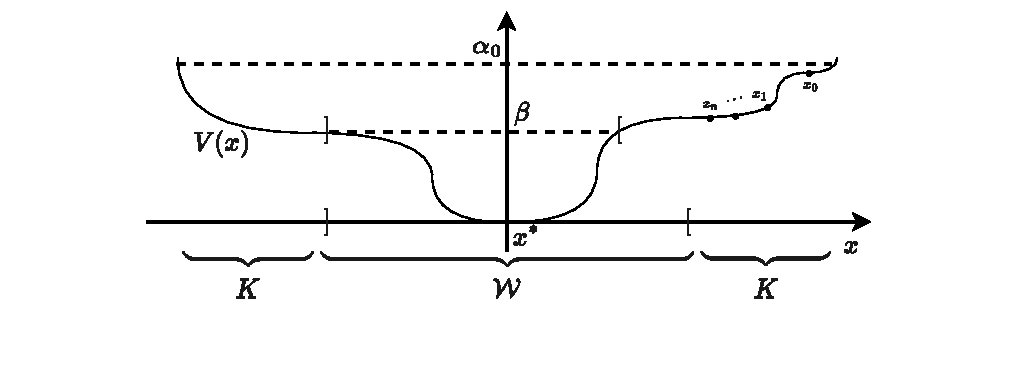
\includegraphics[width=\textwidth,clip,trim=2.2cm 1cm 2.2cm 0]{assets/ljapunov-dim-aff1}
            \caption[Costruzione 1 per teorema di Ljapunov]{Costruzione per dimostrare
            l'affermazione 1.}
            \label{fig:ljapunov-dim-aff1}
        \end{figure}
    \end{minipage}

    Per il teorema di Bolzano-Weierstrass, posso estrarre una
    sottosuccessione di $\{\b x_n\}$ convergente in $K$
    \begin{equation*}
    \{\b x_ {n_k}\} \to \b x.
    \end{equation*}
    Quindi, per la continuità di $V$ vale
    \begin{equation*}
        V(\b x) = 0
    \end{equation*}
    e dalla proprietà (2) della \autoref{def:clf-local}
    segue che
    \begin{equation*}
        \b x = \b x^*.
    \end{equation*}
    Ma questo è un assurdo, visto che che $\b x \in K$
    e $\b x^* \in \mathcal W \subset \bar K$, e prova l'affermazione.

    \hfill\openbox\paragraph{}

    Una conseguenza utile dell'affermazione (1) è che se
    $\xi(t) = \phi^t(\b x, \omega)$ con $t \in [0, +\infty[$ tale che
    \begin{equation*}
        V[\xi(t)] \to 0 \text{ per } t \to +\infty
    \end{equation*}
    allora deve essere
    \begin{equation}
        \xi(t) \to \b x^*.
        \label{eq:xi-to-xstar}
    \end{equation}


    \item Osservo che la proprietà (3) della \autoref{def:clf-local}
    garantisce che per ogni stato $\b y \in \mathcal O$ e $\b y \neq \b x^*$ esiste
    almeno uno stato ben raggiungibile da $\b y$.
    Inoltre vale la proprietà transitiva, ovvero, se $\b y$ è raggiungibile da $\b x$
    e $\b z$ è raggiungibile da $\b y$, allora $\b z$ è raggiungibile da $\b x$.
    Definisco
    \begin{equation*}
        B(\b x) = \inf\left\{ V(\b z)\ |\ \b z \text{ è ben raggiungibile da } \b x \right\}
    \end{equation*}
    e osservo che, per quanto appena detto, vale che $B(x) < V(x)$ per $\b x \neq \b x^*$.
    Dimostro la seguente affermazione.

    \begin{aff}
        \begin{equation*}
            V(\b x) < \alpha_0 \implies B(\b x) = 0,
        \end{equation*}
        dove $\alpha_0$ definisce un insieme compatto, secondo la~\eqref{eq:alpha_0}.
    \end{aff}

    \emph{Dimostrazione}.
    Procedo per assurdo.
    Suppongo che esista un $\b x \neq \b x_0$ per cui $V(\b x) < \alpha_0$
    e $B(\b x) = \alpha > 0$.
    Per come ho scelto $\alpha_0$ deve valere $\b x \in \mathcal O$.
    Considero la successione\footnote{L'esistenza
    è garantita dalla proprietà transitiva della ben raggiungibilità e dal fatto che
    ogni $\b z_n$ ha almneno un elemento che è ben raggiungibile.}
    \begin{equation}
        \{V(\b z_n)\}
        \label{eq:successione-zn}
    \end{equation}
    decrescente dove gli $\b z_n$ sono tutti elementi ben raggiungibili da $\b x$.
    La~\eqref{eq:successione-zn} è limitata da $V(\b z) = \alpha$.
    Tutti gli $\b z_n$ fanno parte del compatto
    \begin{equation*}
        C = \left\{\b z \ |\ V(\b z) \leq V(\b x) \right\}
    \end{equation*}
    e dato che la~\eqref{eq:successione-zn} è monotona e limitata,
    allora è anche convergente e posso fissarne il limite senza perdere
    di generalità:
    \begin{equation}
        \lim_{\b z_n \to \b z} V(\b z_n) = V(\b z) = \alpha.
        \label{eq:vzequalsalpha}
    \end{equation}
    Osservo che
    \begin{equation*}
        \alpha \neq 0 \implies \b z \neq \b x^*
    \end{equation*}
    e che
    \begin{equation*}
        \alpha < V(\b x) < \alpha_0 \implies \b z \in \mathcal O.
    \end{equation*}
    Quindi, deve esistere un $\b y$ che sia ben raggiungibile da $\b z$.
    È importante osservare che, anche se ogni elemento della successione~\eqref{eq:successione-zn}
    è ben raggiungibile da $\b x$, non ho nulla che mi garantisca che $\b z$ lo sia.
    Fisso $\epsilon > 0$ tale che
    \begin{equation}
        V(\b z) < V(\b x) - \epsilon,\ \text{e} \ V(\b y) < V(\b z) - \epsilon
        \label{eq:vy-less-vz}
    \end{equation}
    e prendo $\nu \in \mathcal U^{[0, t[ \subseteq \mathcal T}$ controllo ammesso
    per $\b z$ tale che, detto $\zeta(s) = \phi^s(\b z, \nu)$, valgano
    \begin{align*}
        &\zeta(t) = \b y, \\
        &V[\zeta(s)] \leq V(\b z), \ \forall s \in [0, t[ \subseteq \mathcal T.
    \end{align*}
    La costruzione per la dimostrazione è mostrata in \autoref{fig:ljapunov-dim-aff2}.

    \hfill
    \begin{minipage}{.8\textwidth}
        \begin{figure}[H]
            \centering
            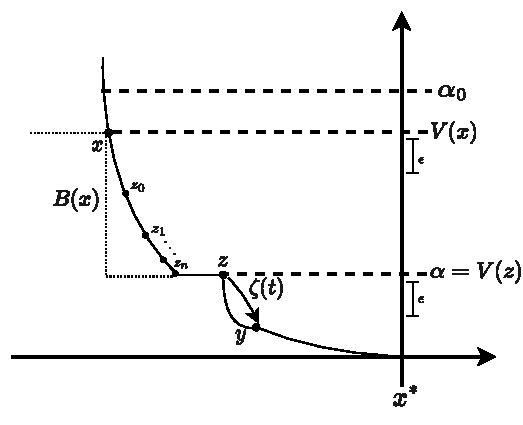
\includegraphics[width=.7\textwidth]{assets/ljapunov-dim-aff2}
            \caption[Costruzione 2 per teorema di Ljapunov]{Costruzione per dimostrare
            l'affermazione 2.}%todo
            \label{fig:ljapunov-dim-aff2}
        \end{figure}
    \end{minipage}

    $V$ è uniformemente continua\footnote{Per ipotesi
        $V$ e continua sul compatto $C$ quindi per il teorema di Heine-Cantor è
        uniformemente continua su $C$.} sul compatto $C$ quindi, fissato $\epsilon >0$ esiste un $\delta > 0$
    tale che, presi $\b a, \b b \in C$
    \begin{equation}
        d(\b a, \b b) < \delta \implies |V(\b a) - V(\b b)| < \epsilon.
        \label{eq:v-uniformemente-continua}
    \end{equation}

    Considero la successione
    \begin{equation*}
        \{V(\b y_n)\}, \text{ con } \b y_n = \zeta_n(t)
    \end{equation*}
    dove $\zeta_n(s) = \phi^s(\b z_n, \nu)$.

    Visto che sto lavorando su uno spazio topologico vale che, fissato $\epsilon > 0$, esiste $\delta > 0$ tale che,
    per valori $n \geq N$ vale
    \begin{equation}
        d_\infty(\zeta_n, \zeta) < \delta \implies d(\b y_n, \b y) < \epsilon,
        \label{eq:phi-continua}
    \end{equation}
    dove $d_\infty$ è la metrica per lo spazio dei controlli ammessi definita da
    \begin{equation*}
        d_{\infty}[\phi^t(\b x, \omega_1), \phi^t(\b x, \omega_2)] =
        \sup \left\{ d[\phi^s(\b x, \omega_1), \phi^s(\b x, \omega_2)],\ s \in \mathcal T  \right\}.
    \end{equation*}
    Ora fisso $\epsilon > 0$ e considero la catena di implicazioni data
    dalla~\eqref{eq:v-uniformemente-continua} e dalla~\eqref{eq:phi-continua}:
    \begin{equation}
        d_\infty(\zeta_n, \zeta) < \delta' \implies d(\b y_n, \b y) < \delta \implies |V(\b y_n) - V(\b y)| < \epsilon
        \label{eq:implication-chain}
    \end{equation}
    da cui
    \begin{equation}
        \left| V[\zeta_N(s)] - V[\zeta(s)] \right| < \epsilon\ \forall s \in [0, t].
        \label{eq:lesser-forall-t}
    \end{equation}

    Dimostro che $\b y_N$ è ben raggiungibile da $\b x$.
    È sufficiente dimostrare che
    \begin{equation*}
        V[\zeta_N(s)] < V(\b x)\  \forall s \in [0, t].
    \end{equation*}
    Considero la~\eqref{eq:lesser-forall-t} e applico la definizione di modulo (studio entrambi i casi).
    \begin{itemize}
        \item Caso $V[\zeta(s)] < V[\zeta_N(s)]$:
            \begin{align*}
                V[\zeta_N(s)] - V[\zeta(s)] &< \epsilon \\
                V[\zeta_N(s)] &< \epsilon + V[\zeta(s)] \\
                V[\zeta_N(s)] &< \epsilon + V(\b z) \\
                V[\zeta_N(s)] &< V(\b x) \numberthis\label{eq:modulo-caso-1}
            \end{align*}
            dove nell'ultimo passaggio ho applicato la~\eqref{eq:vy-less-vz}.
        \item Caso $V[\zeta(s)] > V[\zeta_N(s)]$:
            \begin{align*}
                V(\b x) > V(\b z) > V[\zeta(s)] > V[\zeta_N(s)]. \numberthis\label{eq:modulo-caso-2}
            \end{align*}
    \end{itemize}
    Chiamo $\omega$ la legge di controllo che porta $\b x$ a $\b z_N$.
    Per la proprietà di composizione della mappa di transizione, posso concatenare
    $\omega$ con $\nu$, in modo da ottenre una legge di controllo che porti $\b x$ a $\b y_N$.
    Questo, unito al fatto che la~\eqref{eq:modulo-caso-1} e la~\eqref{eq:modulo-caso-2}
    valgono per $s \in [0, t]$, è sufficiente a dimostrare che $\b y_N$ è ben raggiungibile da $\b x$.

    In questo modo cado in assurdo visto che la~\eqref{eq:implication-chain}
    unita alla~\eqref{eq:vy-less-vz} e alla~\eqref{eq:vzequalsalpha} implicano
    che $V(\b y_n) < B(\b x)$, violando la tesi.
    L'assurdo è dato dall'aver assunto che $\alpha = B(\b x) > 0$.

    \hfill \openbox \paragraph{}

    L'andamento di $B(\b x)$ è mostrato in \autoref{fig:ljapunov-aff2}.

    \hfill
    \begin{minipage}{.8\textwidth}
        \begin{figure}[H]
                \centering
                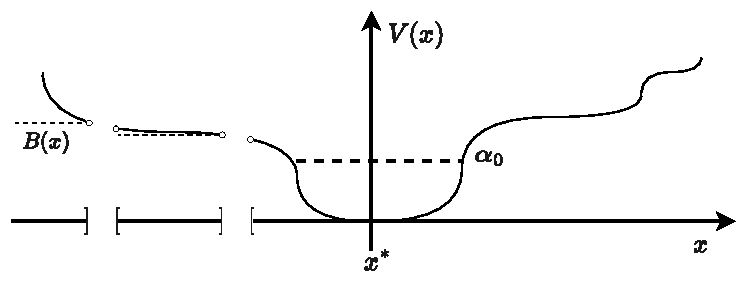
\includegraphics[width=\textwidth]{assets/ljapunov-aff2}
                \caption[Andamento di $B(\b x)$]{Andamento di $B(x)$ per uno
                spazio delle fasi monodimensionale. La funzione è a tratti e
                si annulla dentro al compatto più grande contenente $x^*$.}
                \label{fig:ljapunov-aff2}
        \end{figure}
    \end{minipage}

    \item Dimostro che vale la seguente affermazione

    \begin{aff}
        Se $V(\b x) < \alpha_0$ con $\b x \neq \b x^*$ allora esiste
        una sequenza di stati
        \begin{equation*}
        \{\b x_n\}
        \end{equation*}
        con $\b x_0 = \b x$, una sequenza di tempi
        \begin{equation*}
        t_n \in \mathcal T
        \end{equation*}
        e una sequenza di controlli
        \begin{equation*}
            \omega_n \in \mathcal U^{[0, t_n[ \in \mathcal T}
        \end{equation*}
        tale che valgano le seguenti proprietà
        \begin{itemize}
            \item $\omega_n$ è ammesso per $\b x_n$.
            \item $\phi^{t_n}(\b x_n, \omega_n) = \b x_{n+1}$
            \item Con $\xi_n(t) = \phi^t(\b x_n, \omega_n)$ vale $V[\xi_n(t)] \leq \frac 1 {2^n} V(\b x), \ \forall t \in [0, t_n]$
        \end{itemize}
    \end{aff}
    \emph{Dimostrazione}.
    Procedo per induzione.
    Voglio dimostrare che  per ogni $\b x \in \Sigma$ tale che
    \begin{equation*}
        0 < V(\b x) < \alpha_0
    \end{equation*}
    esiste un certo tempo $t > 1$ e un controllo $\omega$
    di lunghezza $t$ ammesso per $\b x$ tale che
    \begin{align*}
        V[\xi(s)] &\leq V(\b x) \text{ con } s \in [0, t], \\
        V[\xi(t)] &< \frac 1 2 V(\b x).
    \end{align*}
    Per continuità di $V$ in $\b x^*$, esiste un $\epsilon > 0$ per cui
    \begin{equation}
        d(\b z, \b x^*) < \epsilon \implies V(\b z) < \frac 1 2 V(\b x).
        \label{eq:dzxstar}
    \end{equation}
    Sia $\omega_0 \in \mathcal U^{[0, 1[}$ il controllo nullo,
    tale che
    \begin{equation*}
        \phi^s(\b x^*, \omega_0) = \b x^*.
    \end{equation*}
    Visto che sto lavorando in uno spazio topologico
    esiste un $\delta > 0$ tale che, fissato $\epsilon > 0$ e
    dato $\zeta(s) = \phi^s(\b y, \omega_0)$,
    \begin{equation*}
        d(\b y, \b x^*) < \delta \implies d(\zeta(s), \b x^*) < \epsilon
    \end{equation*}
    e $\omega_0$ è ammesso per $\b y$ per $s \in \mathcal T$.

    Per la~\eqref{eq:dzxstar} posso scegliere $\epsilon$ in modo che
    \begin{equation*}
        V[\zeta(s)] < \frac 1 2 V(\b x)
    \end{equation*}
    valga per $s \in [0, 1]$.
    Per l'affermazione (1) esiste $\delta_0 > 0$ tale che
    \begin{equation}
        V(\b y) < \delta_0 \implies d(\b y, \b x^*) < \delta.
        \label{eq:vylessdelta0}
    \end{equation}
    Per l'affermazione (2), vale $B(\b x) = 0$.
    Quindi esiste un controllo $\omega_1$ e un tempo $t_1$ tale
    che, dato $\xi_1 = \phi^{t_1}(\b x, \omega_1)$, vale
    \begin{align*}
        V[\xi_1(s)] &\leq V(\b x), \text{ con } s \in [0, t_1],\\
        V[\xi_1(t_1)] &< \delta_0
    \end{align*}
    e, per la~\eqref{eq:vylessdelta0}, vale anche
    \begin{equation*}
        d[\xi_1(t_1), \b x^*] < \delta.
    \end{equation*}
    La costruzione per la dimostrazione è mostrata in \autoref{fig:ljapunov-dim-aff3}.

    \hfill
    \begin{minipage}{.8\textwidth}
        \begin{figure}[H]
            \centering
            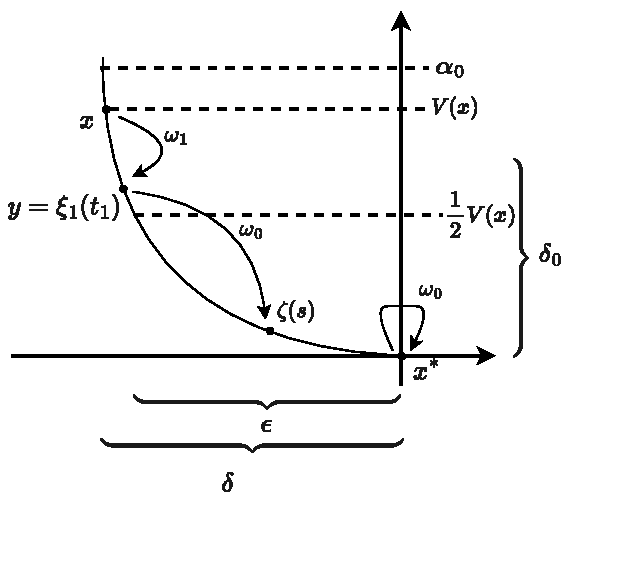
\includegraphics[width=.8\textwidth]{assets/ljapunov-dim-aff3}
            \caption[Costruzione 3 per teorema di Ljapunov]{Costruzione per dimostrare
            l'affermazione 3.}%todo
            \label{fig:ljapunov-dim-aff3}
        \end{figure}
    \end{minipage}

    La sequenza che cerco è quindi data dalla concatenazione di
    $\omega_1$ e $\omega_0$ opportunamente traslati.

    \hfill\openbox\paragraph{}

    L'affermazione (3) mi permette di definire una legge di controllo
    $\omega$ su $[0, +\infty[ \subseteq \mathcal T$ ammessa per $\b x$
    data dalla concatenazione degli $\omega_n$.
    Detta quindi $\xi(t) = \phi^t(\b x, \omega)$ vale
    \begin{equation*}
        V[\xi(t)] \to 0 \text{ per } t \to +\infty
    \end{equation*}
    e per la~\eqref{eq:xi-to-xstar} vale
    \begin{equation}
        \xi(t) \to \b x^*.
        \label{eq:xi-to-xstar-2}
    \end{equation}

    \item Dimostro che il sistema è localmente asintoticamente
    controllabile.
    Prendo $\mathcal V$ un intorno di $\b x^*$, prendo $\alpha_1$ tale che
    \begin{equation}
     \{\b y\ |\ V(\b y) < \alpha_1 \} \subseteq \mathcal V
        \label{eq:def-alpha1}
    \end{equation}
    e definisco
    \begin{equation*}
        \alpha = \min\{\alpha_0, \alpha_1\}.
    \end{equation*}
    Nella definizione di localmente asintoticamente controllabile prendo
    \begin{equation*}
            \mathcal W = \{\b y\ |\ V(\b y) < \alpha\}.
    \end{equation*}

    L'affermazione (3) è valida per ogni $\b y \neq \b x^* \in \mathcal W$
    dato che $V(\b y) < \alpha_0 \leq \alpha$.
    Quindi, per la~\eqref{eq:xi-to-xstar-2} esiste un controllo $\omega$
    su $\mathcal T$ tale che
    \begin{align*}
        &\phi^0(\b y, \omega) = \b y, \\
        &\phi^t(\b y, \omega) \to \b x^* \text{ per } t \to +\infty
    \end{align*}
    e per la~\eqref{eq:def-alpha1} vale anche
    \begin{equation*}
        \phi^t(\b y, \omega) \in \mathcal V, \ t \in [0, +\infty[ \subseteq \mathcal T.
    \end{equation*}
    quindi il sistema è localmente asintoticamente controllabile.

    \hfill\qedsymbol\paragraph{}

    \item Dimostro che il sistema è asintoticamente controllabile.
    Assumo che $V$ sia una funzione di controllo di Ljapunov globale
    e prendo $\b y \in \Sigma$.
    Sia $\beta = V(\b y)$.
    Ora osservo che nella dimostrazione fatta fino ad ora posso prendere
    $\mathcal O = \Sigma$ e $\alpha_0 = \beta + 1$
    senza perdere di generalità, in quanto l'unica proprietà che $\mathcal O$
    e $\alpha_0$ devono rispettare è che l'insieme $C$
    definito nella~\eqref{eq:alpha_0}
    sia compatto e contenuto in $\mathcal O$.
    Quindi, se nel passaggio (4) prendo $\mathcal V = \Sigma$
    posso prendere $\alpha_1 = \beta + 1$ in modo che
    $\b y \in \mathcal{W}$ e che il sistema sia
    asintoticamente controllabile a $\b x^*$.

    \hfill\qedsymbol\paragraph{}

\end{steps}

Concludo questo capitolo dicendo che è possibile
dimostrare la seguente proposizione.
\begin{prop}
    Sia dato uno spazio topologico in cui è 
    definita una funzione $V : \Sigma \to \R$ continua.
    Sia $\mathcal O \subseteq \Sigma$
    un insieme aperto per cui la restrizione di
    $V$ su $\mathcal O$ sia differenziabile con 
    continuità e valgano le proprietà (1) e (2) 
    della \autoref{def:clf-local}.
    Allora, una condizione sufficiente perchè $V$
    sia una funzione di controllo di Ljapunov locale è che per ogni $\b x \neq \b x_0 \in \mathcal O$
    esista un controllo $\omega$ tale che
    \begin{equation*}
        \frac{dV(\phi^t(\b x, \omega))}{dt} < 0.
    \end{equation*}
    Se questa proprietà vale per $\mathcal O = \Sigma$, $V$ è una funzione di controllo di Ljapunov globale. 
    \label{prop:condizione-sufficiente-ljapunov}
\end{prop}
La dimostrazione si trova in~\cite{sontagMath}.